\documentclass{standalone}


\begin{document}

\subsection[Sorting]{Pair sort}\label{implementation:sort}

The sorting algorithm starts at the end of variable couple evaluation and re-order the pairs in ascending order to ease the next steps of signature identification\footnote{
  We are talking about couples performances meaning the classification accuracy of the feature pair up to now.
  In some cases the simple accuracy is useless, especially when we are working with unbalanced population classes.
  In this case we can use a statistical score which takes in count the balanced between the right classifications of our samples (e.g Matthews Correlation coefficient, MCC).
  The developed code evaluate either the global accuracy of classification either the MCC and, with slight changes allows to perform the re-ordering of feature pair according to the desired score.
  Since in the next section we will discuss the application of the DNetPRO algorithm to real data using only the classification accuracy as score, we focused only on it in the next sections.
}.
This step is performed in the same code (and same parallel section) of the previous section but it deserves an own topic for a better focus on the parallelization strategy chosen.
Moreover, there are many common parallel implementation of sorting algorithm and, to reach the best performances, we have to chose the appropriated one.

The sorting algorithm are already implemented in serial version in the major part of the languages (\textsf{Python} and \textsf{C++} included).
The naive version of the algorithms are also quite optimized and they perform the computation with complexity $(O(N\dot\log(N)))$\footnote{
  We are considering only un-stable sort in which the preserving order of equivalent elements in the array is not guaranteed.
}.
In this case we have not to re-invent any sorting technique but only insert as well as possible these algorithms inside a parallel sections and use the variable format chosen for couple performances storage.
Since we are working with SoA objects we need to re-order all the structure arrays in the same way.
So we can not use a simple sort function but can compute the set of indexes that allow the re-order of the arrays, the so called \textsf{argsort} method.
To rearrange the indexes according to a given array of values we can use the templates in \textsf{C++}.

\begin{figure}[htbp]
\centering
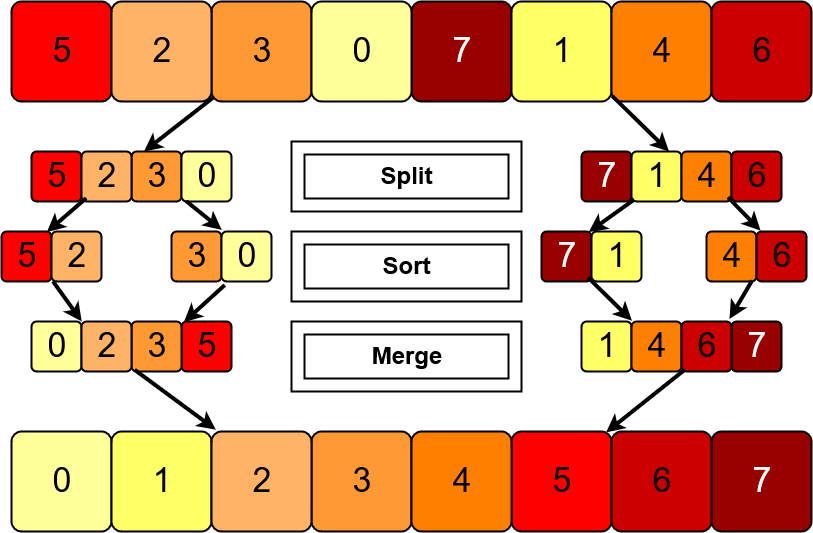
\includegraphics[width=0.45\textwidth]{merge_sort.png}
\caption{Parallel merge-sort algorithm scheme.
Starting from the original array, the master thread splits the work (sub-arrays) along two slave threads (\textsf{split} step in the graph).
The split recursion is applied until a required size of sub-arrays is reached.
Each slave-thread applies a sort function (\textsf{sort} step in the graph).
Then, the full array is recombined following back the thread recursion and applying an \textsf{inplace-merge} function (\textsf{merge} step in the graph).
}
\label{fig:merge_sort}
\end{figure}

As parallelization strategy we can yet invoke the new \emph{keywords} of OpenMP libraries and apply a \emph{divide-and-conquer} architecture using a tree of independent \textsf{tasks}\footnote{
  Tasks in OpenMP are code blocks that the compiler wraps up and makes available to be executed in parallel.
}.
Using the maximum power of two of the available threads, we split the computation in equal size sub-arrays and perform independent \textsf{argsort}s.
Then, going backwards to the subdivisions at each step, we merge the sub-arrays two-by-two until the root (ref Fig.~\ref{fig:merge_sort}).


\end{document}
